This section shows the characterization of no-clad BCF-12 fibers from Saint Gobain, which are the fibers used in the TRITIUM experiment. These measurements are compared to other measurements that have been made using single clad and multiclad BCF-12 fibers to quantify how the clad affect to several parameters of scintillating fibers.

It is an interesting comparison because, although commercial clads cannot be used for the TRITIUM experiment, we can develop our own clad with a low enough thickness. For example, clads with a thickness of the order of tens of nanometers can be achieved by electrodeposition techniques.

As we have seen in the section \ref{subsec:PlasticScintillators}, the difference between these three types of fibers is that no clad fibers only consist of a polystyrene core with a refractive index of $1.60$ whereas, in single clad fibers, the polystyrene core has an acrylic cover (PMMA) with a thickness of $30~\mu\meter$ and a refractive index of $1.49$ and, in multiclad fibers, this acrylic cover has another fluor-acrylic cover with a thickness of $10~\mu\meter$ and a refractive index of 1.42.

%The first measurement that was made is the measurement of the diameter of the fiber. It is important because scintillating molecules are only present in the polystyrene core and we need to know whether the entire polystyrene core is the same size or not. Three different samples of each type of fiber were measured and the results are presented in table \ ref {}.

%TABLAAA DIAMETROOOS

%Therefore, we can see that all fibers have the same external size, which means that the diameter of the polystyrene core is smaller for single clad fibers ($0.97~\mm$) and even smaller for multiclad fibers ($0.96~\mm$). It is an important result since...

This characterization has been carried out at the level of a single scintillating fiber and the parameters that have been measured in every type of fiber are the fiber collection efficiency and the uncertainty in the fiber response due to the conditioning process developed in TRITIUM. The reference measure that will be used for that is the number of photons per second that reach the active area of the photosensor.
%r8520-406

To measure this parameter we will use a calibrated PMT, model R8520-06SEL, whose quantum efficiency at the working wavelength, $29.76\%$, has been measured by Hammamatsu. As we have seen in the section \ref{subsubsec:PMTsElectronicalSystem}, to measure this parameter, on the one hand, we need to work without internal gain of the PMT and, for this task, we will use the PCB described in the section \ref{subsubsec:PMTsElectronicalSystem}, figure \ref{fig:PMTBaseWithoutGain} and, on the other hand, the Keithley 6487 Picoammeter/Voltage Source will be used to measure the output current of the PMTs. The number of photons per second can be known from the Keithley measurement using the equation \ref{eq:NumPhotonsFromIntensityPMT} with $QE=0.2976$ and $CE=1$. The figure \ref{fig:SetUpFiberCharacterization} shows a schematic of the set up used for this characterization.

\begin{figure}[h]
\centering
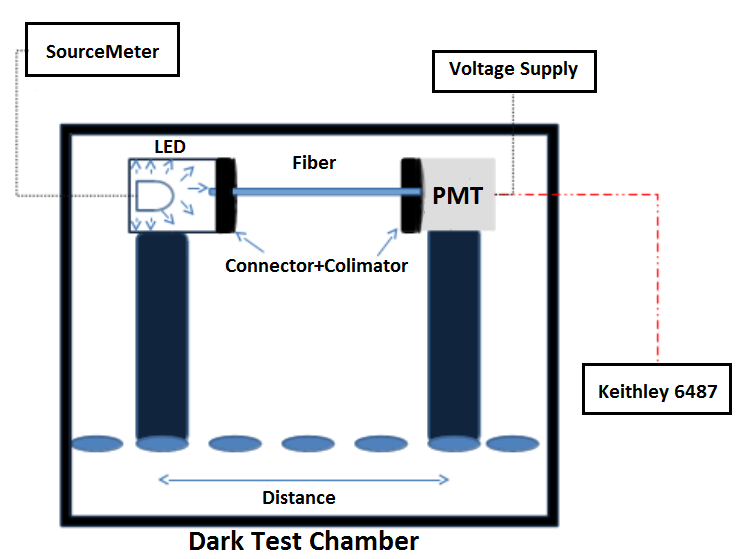
\includegraphics[scale=0.6]{4ResearchAndDevelopments/41Fibers/SetUp_Fiber_Characterization.png}
\caption{Set up used for fiber characterization.\label{fig:SetUpFiberCharacterization}}
\end{figure}

It consists of an optical structure in which a LED and a PMT are fixed to the specific distance between them, established by the user. The LED used is the model LED435-03 from the Roithner LaserTechnik Gmbh company \cite{LEDRLT}, whose emission spectrum is shown in figure \ref{fig:LEDSpectrumTritium}, which has been experimentaly measured using a spectrometer and fitted to a Gaussian function. We can see that the emission peak of this LED is produced at $433.9~\nano\meter$ with a FWHM of $18.4~\nm$. With this LED we intend to simulate the light emission by the fibers used in the TRITIUM experiment, similar to how we explained in section \ref{subsubsec:SiPMsElectronicalSystem}.

\begin{figure}[h]
\centering
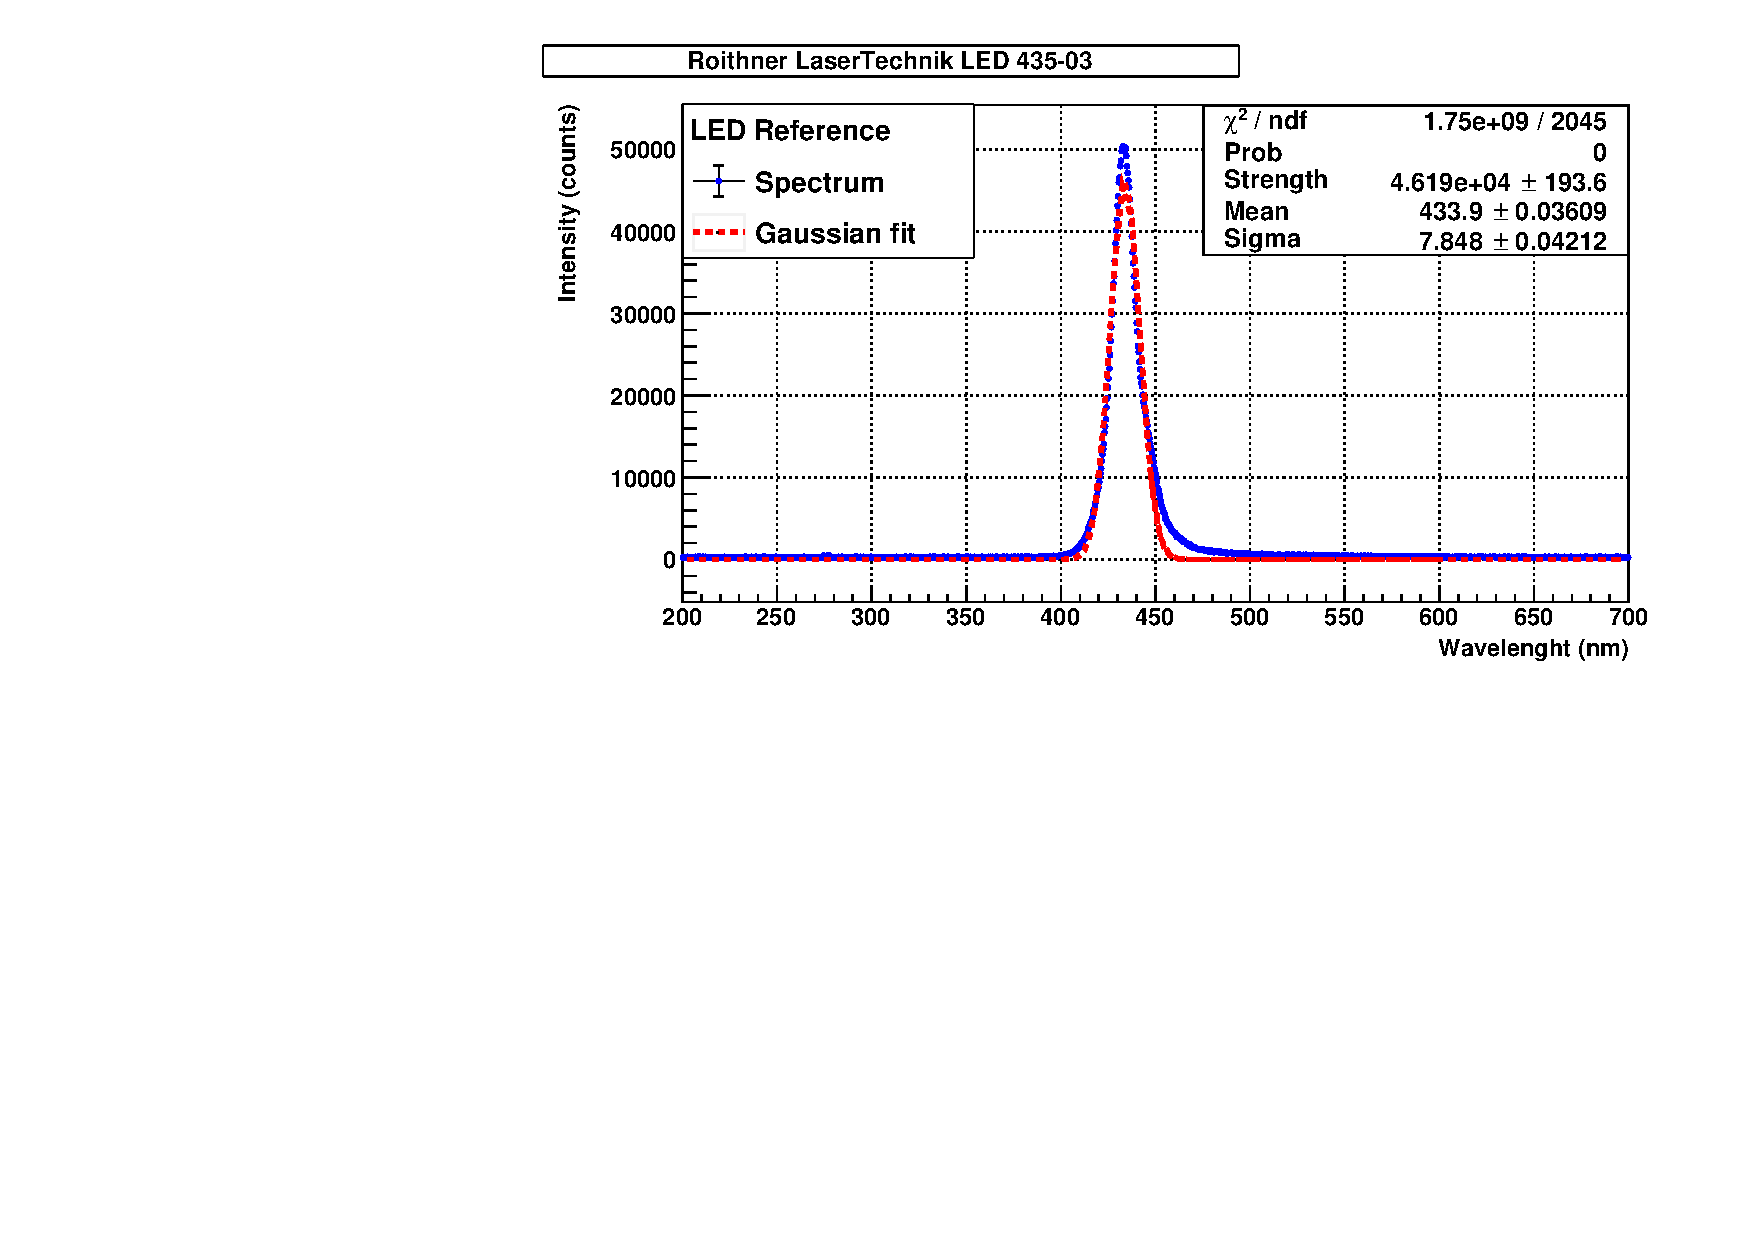
\includegraphics[scale=0.6]{4ResearchAndDevelopments/41Fibers/LED_TRITIUM.pdf}
\caption{Emission spectrum measured for the LED model 435-03 from Roithner LaserTechnik Gmbh Company.\label{fig:LEDSpectrumTritium}}
\end{figure}

The fiber will be fixed between the LED and the PMT, whose distance will be configured based on the length of the fiber, $20~\cm$ for all this study, and optic grass will be used for optimal optical coupling between the fiber and the PMT. Two collimators are used to ensure that the photons detected in the PMT are only those that come from the LED and travel through the fiber and two connectors, type FH-ST\footnote{FH-ST is a quick assembly connector for $1~\mm$ POF} from RoHS company \cite{}, were placed to the ends of the fiber and used to fix it to the system. 

Before we start with the characterization of the fiber we have to perform several tasks to check that our system is fully prepared to measure. On the one hand we have to verify the quality of the tightness to the light of the black box used and, on the other hand, we have to verify the correct operation of the PMT for this study, which involves checking the correct operation of the PCB designed to work without internal gain and checking the linearity of the PMT output signal in the study range.

First, the quality of the light tightness of the black box used will be verified. It is important because we are detecting a few hundred photons per nanosecond, so we must check that our background is as small as possible.

This test will be carried out by measuring a no-clad fiber, whose length is $20~\cm$, in the previous assembly. This measurement was carried out by feeding the LED with four different intensities ($0.05~\milli\ampere$, $0.1~\milli\ampere$, $0.15~\milli\ampere$ and $0.2~\milli\ampere$) and this measurement will be repeated covering the set up with a special black blanket from Thorlabs \cite{BlackBlancket} with which we can make sure that the amount of photons that reach our system is negligible. 

This test was repeated for three different no clad fiber samples and the mean and standard deviation were calculated using the equations \ref{eq:MeanAndStandardDesviation}.

\begin{equation}
\bar{x}=\frac{\sum_{i=0}^{N}x_i}{N}; \qquad Std.~Des. = \frac{\sqrt{\sum_{i=0}^{N}(x_i-\bar{x})^2}}{N-1};
\label{eq:MeanAndStandardDesviation}
\end{equation}

The difference between the results obtained in both tests is presented in the figure \ref{fig:LightTightnessTest}.

%\begin{figure}[]
 %\centering
  %\subfloat[The measurement obtained by covering the setup with a special black blanket and not covering.]{
   %\label{subfig:LightTightnessTestData}
    %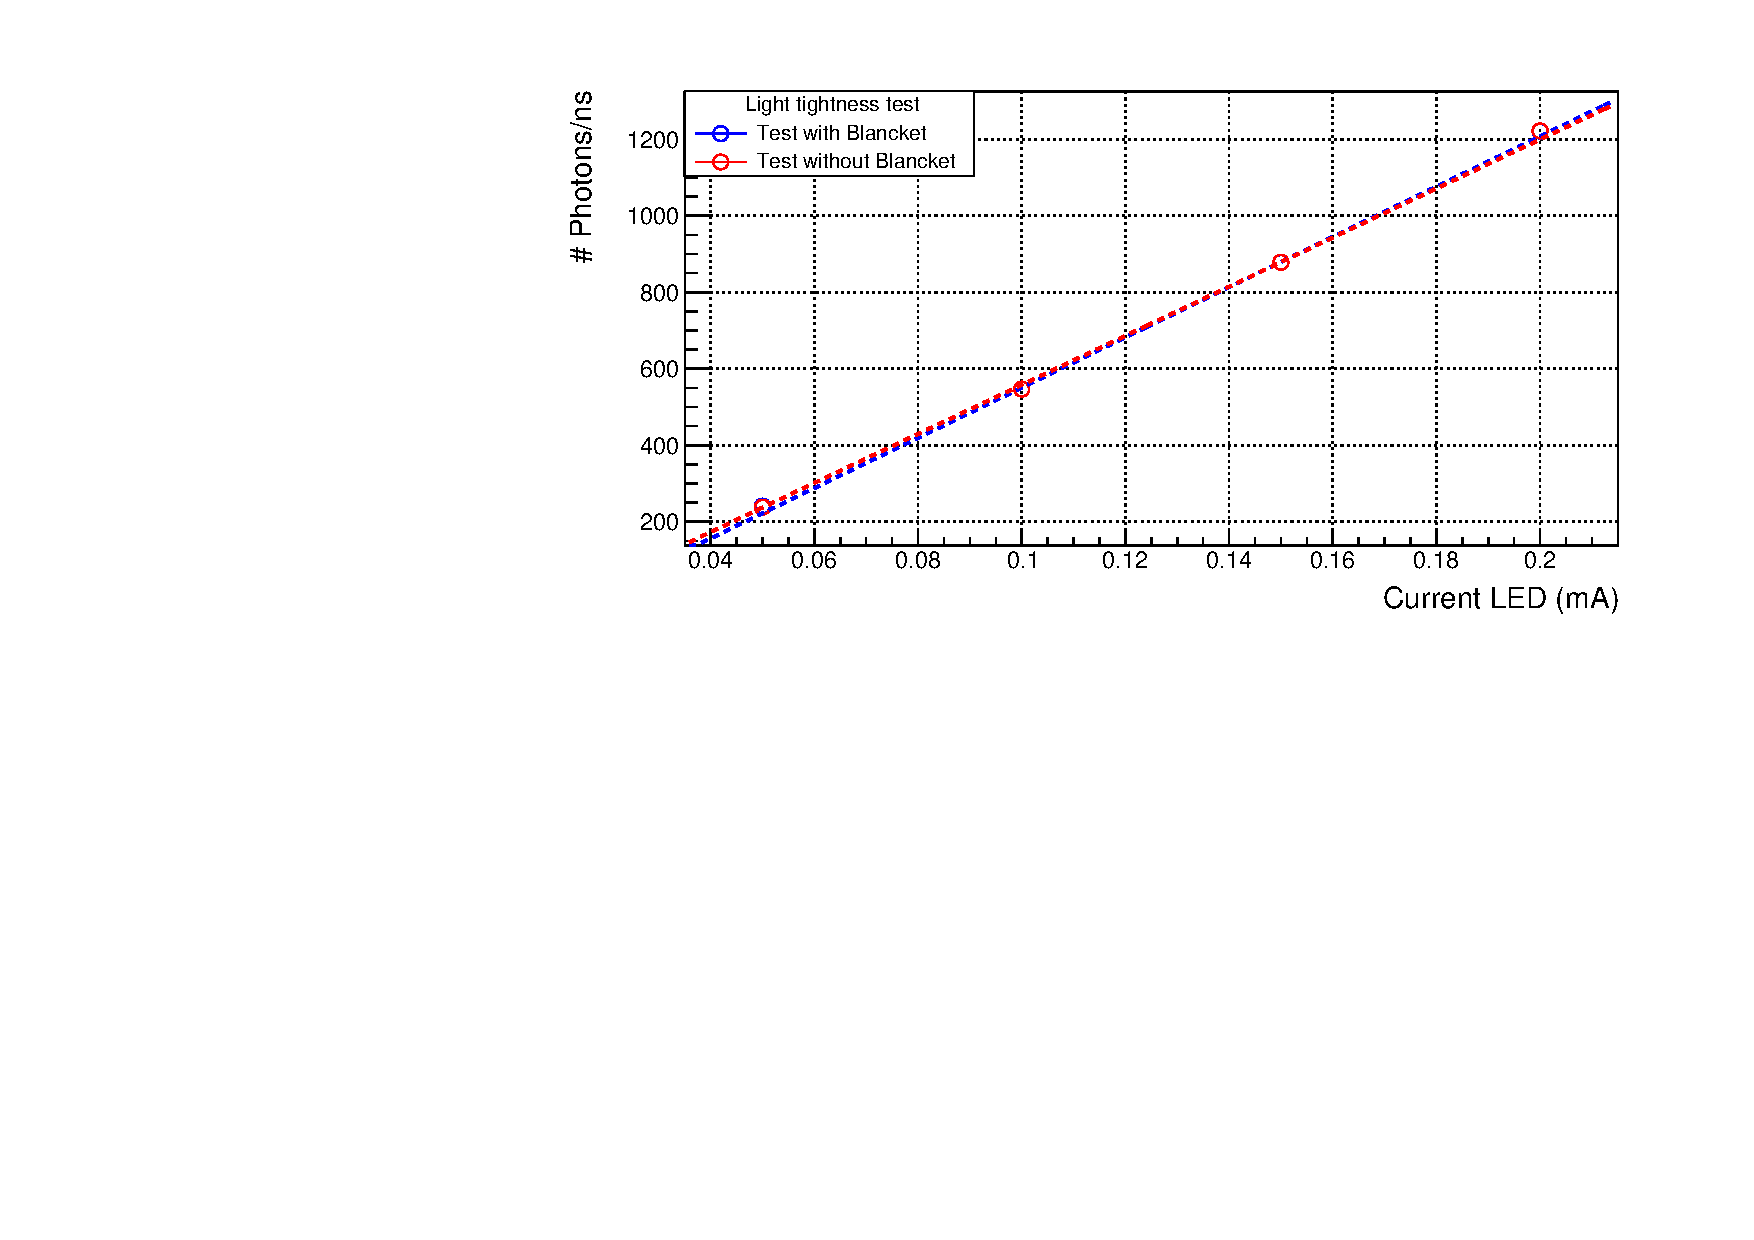
\includegraphics[width=0.9\textwidth]{4ResearchAndDevelopments/41Fibers/Light_tightness_Measurements.pdf}}
    %\newline
  %\subfloat[.]{
   %\label{subfig:LightTightnessTestDifference}
    %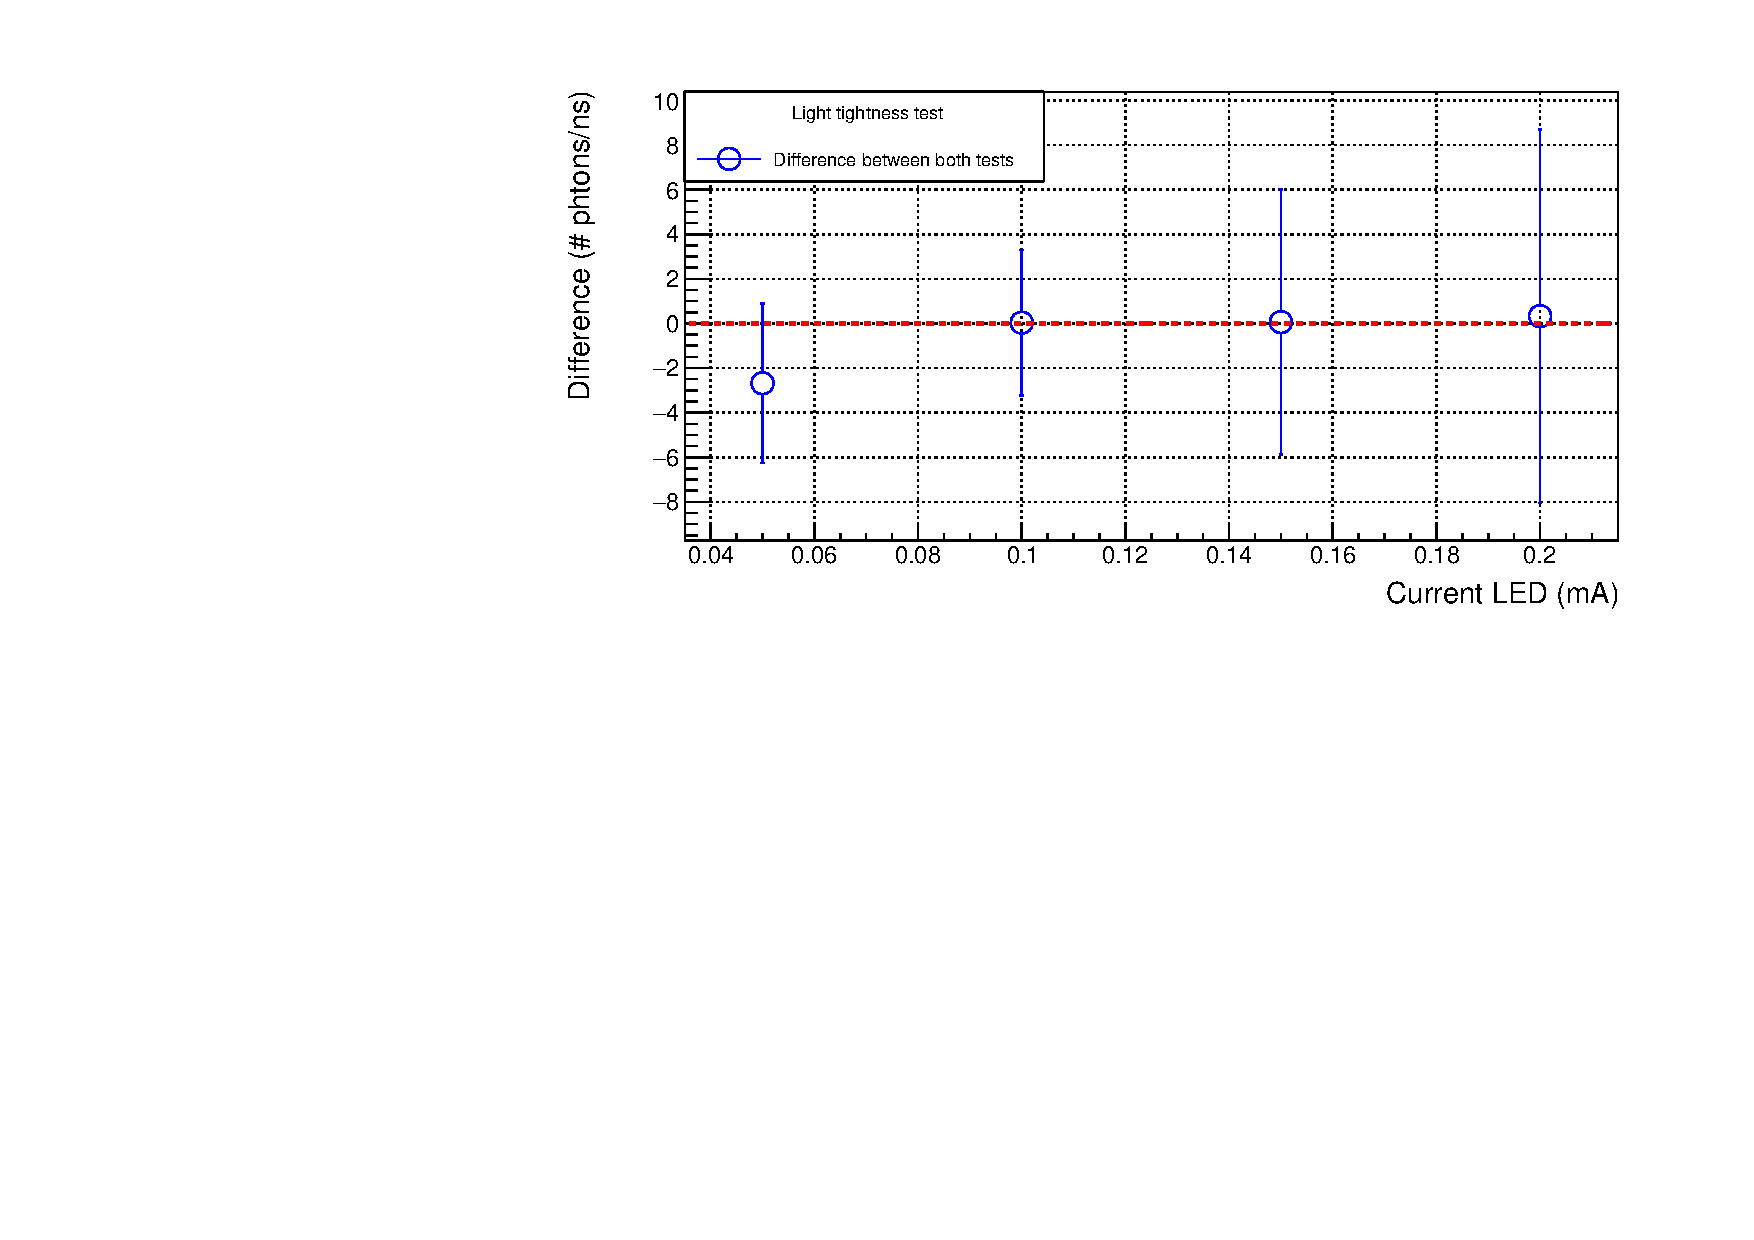
\includegraphics[width=0.9\textwidth]{4ResearchAndDevelopments/41Fibers/Light_tightness_difference.pdf}}
 %\caption{Energy spectrums used to test the effect of the Polishing machine}
 %\label{fig:LightTightnessTest}
%\end{figure}

\begin{figure}[h]
\centering
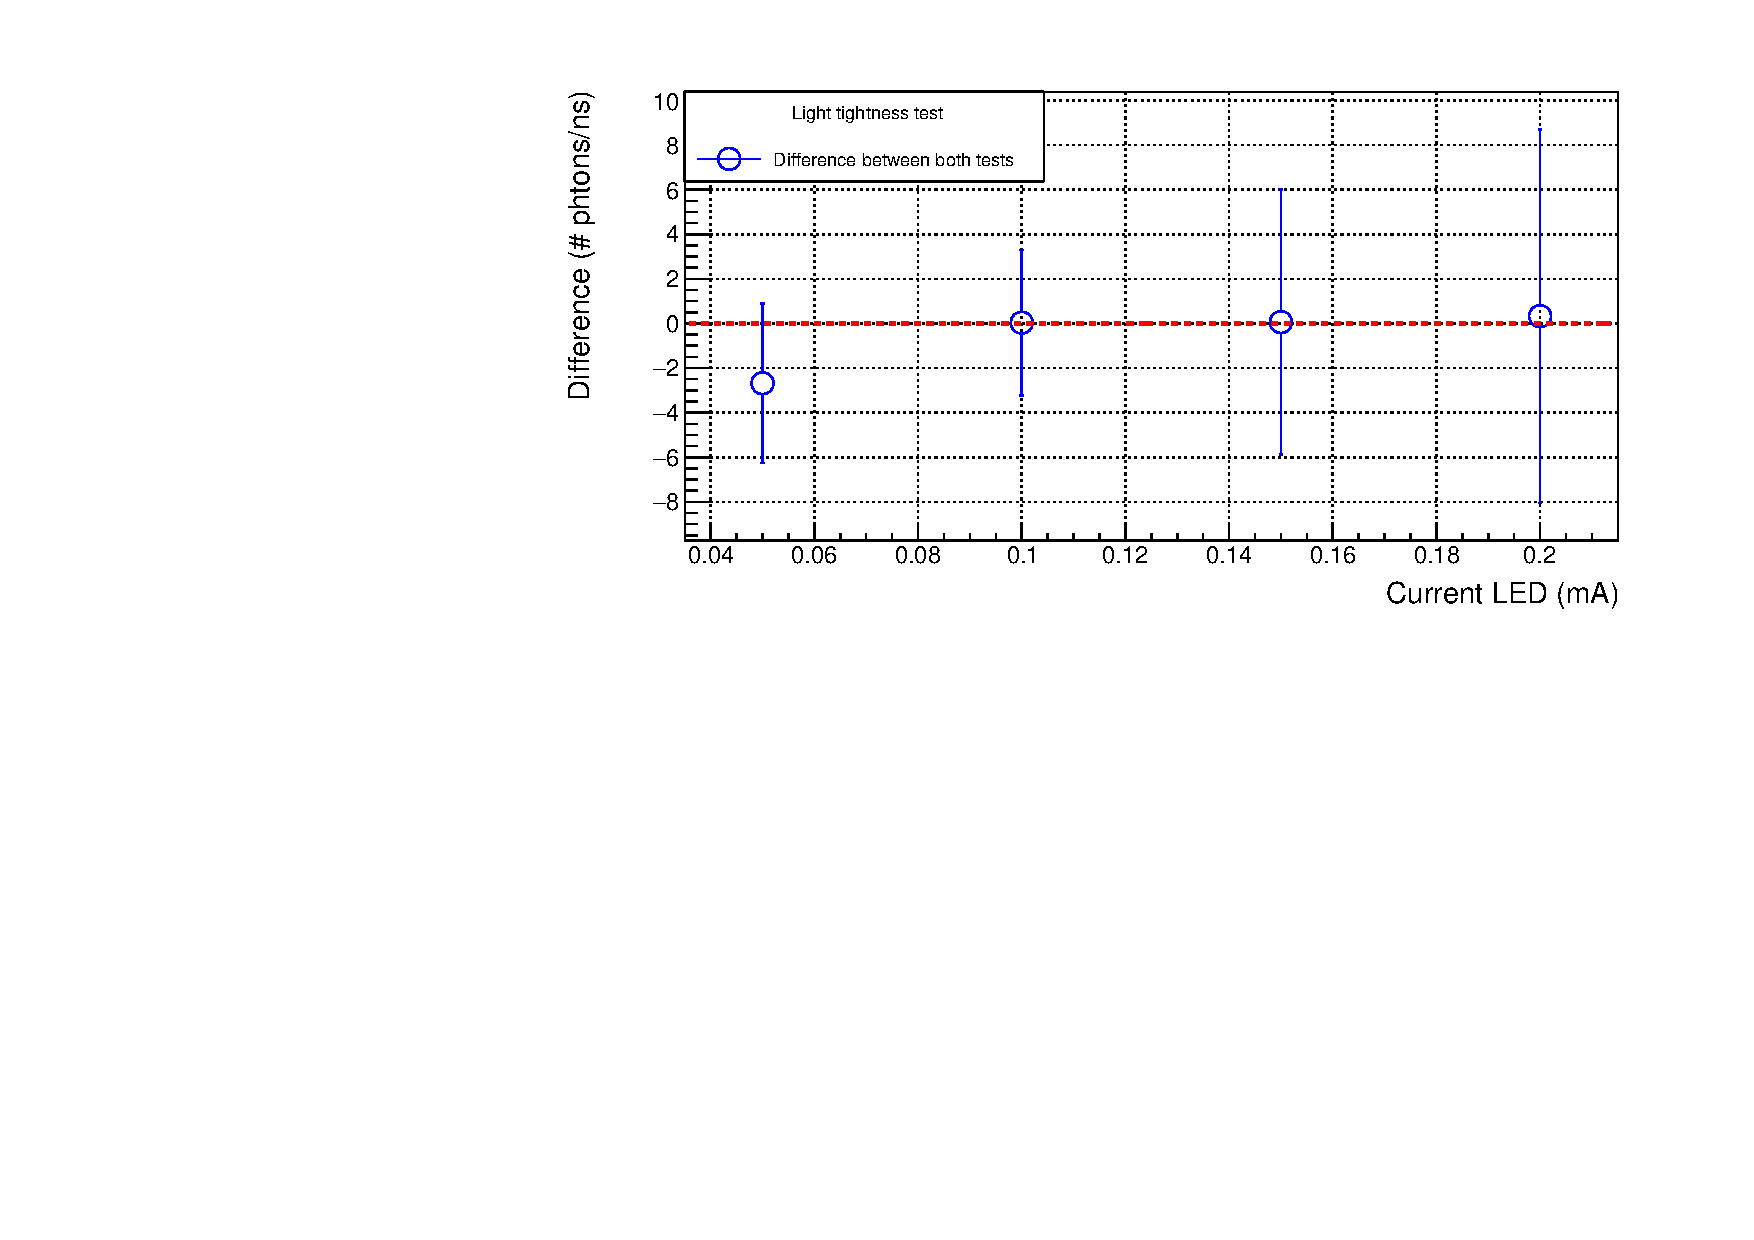
\includegraphics[scale=0.6]{4ResearchAndDevelopments/41Fibers/Light_tightness_difference.pdf}
\caption{Difference between the results obtained in both tests carried out to check the light-tight quality of the system.\label{fig:LightTightnessTest}}
\end{figure}

As can be seen in this figure, there are no statistically relevant differences between both situations, which can be verified with the help of the red auxiliary line that marks 0 (no difference). Therefore, we can be sure that the quality of the light tightness of the black box used is high enough for our tests.

Then the operation of the PCB without the internal gain will be tested. It consists of finding the plateau in which the electron collection efficiency in the first dynode is practically $100\%$. 

This test will consist of, using the setup previously explained without any fiber, feeding the LED at $1~\milli\ampere$ intensity. There, the PMT output current was measured for different voltages between $0$ and $500~\volt$. The figure \ref{fig:PlateauNoGainPMT} show the number of photons detected by the PMT (using a semi logarithmic scale).

\begin{figure}[h]
\centering
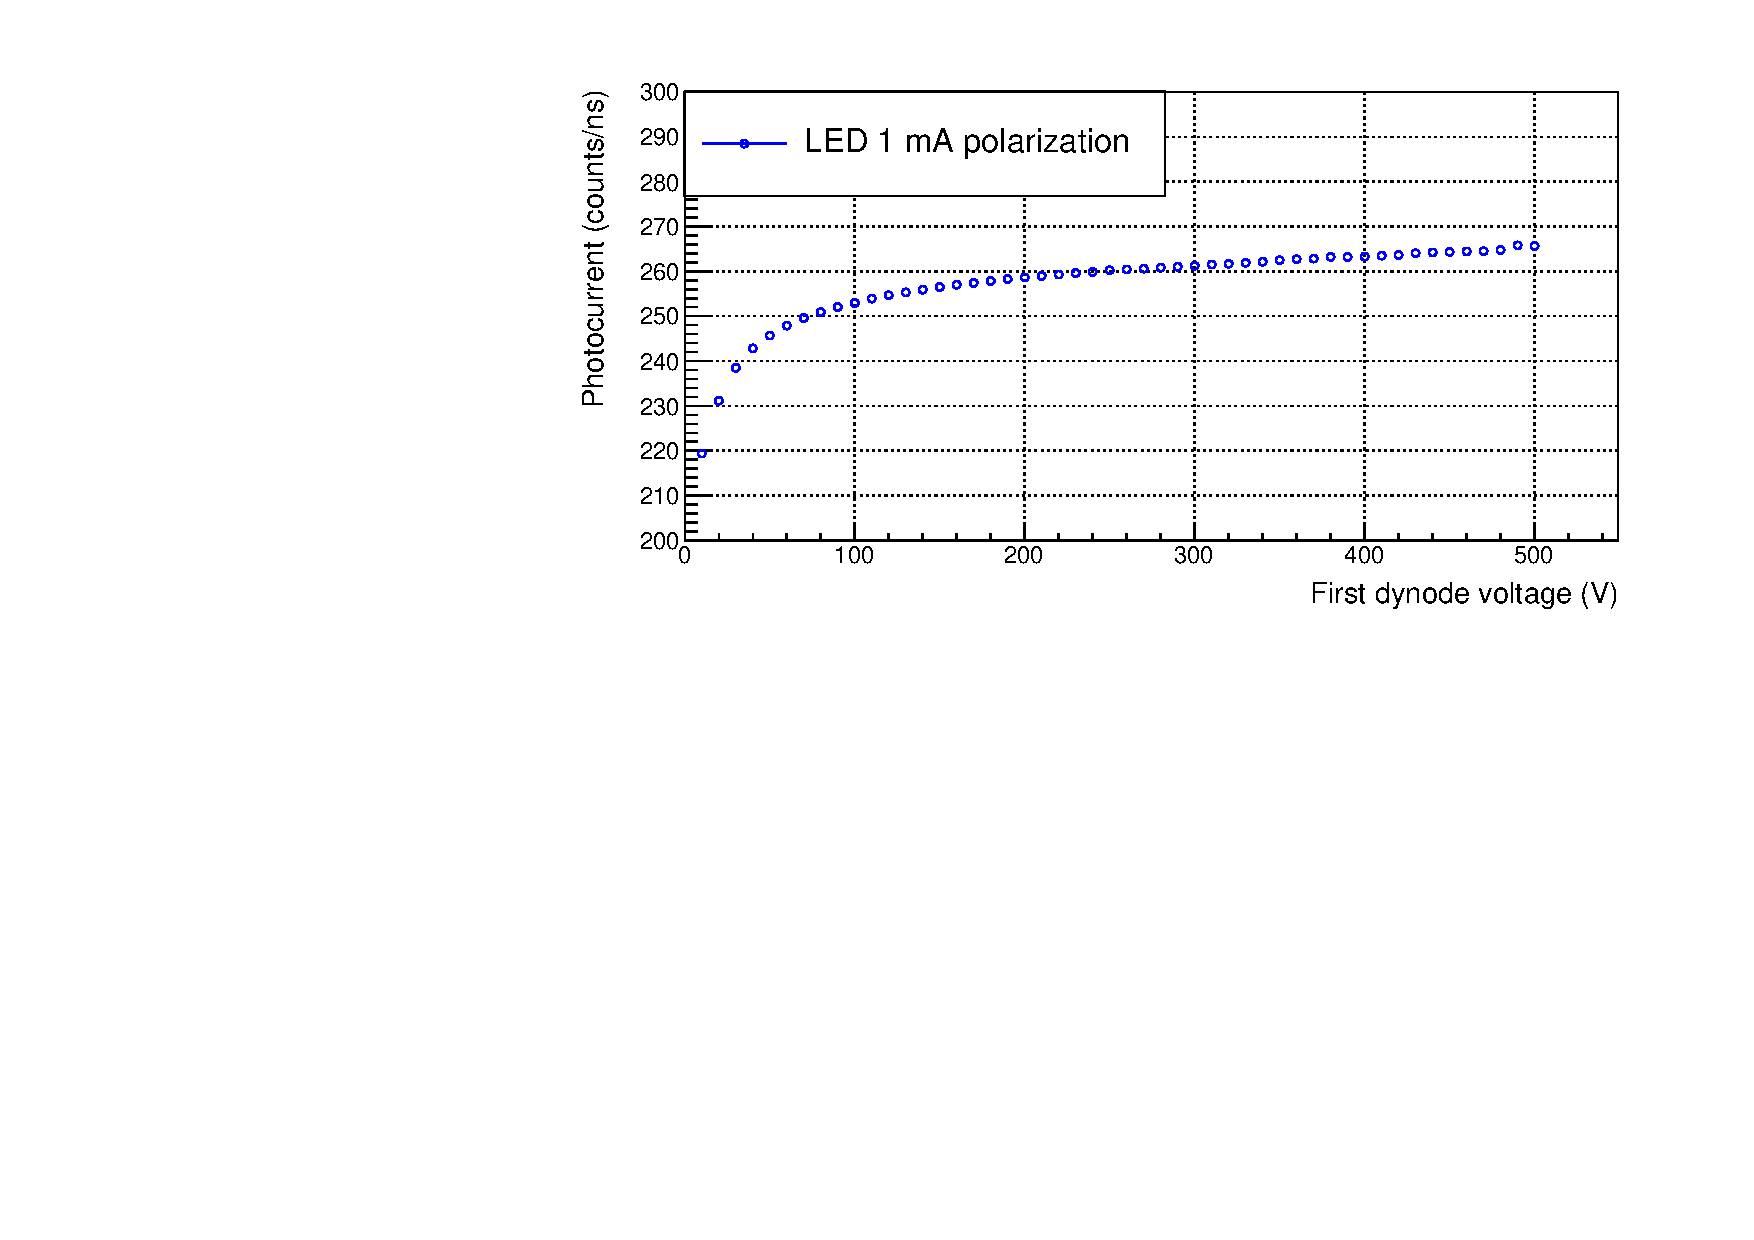
\includegraphics[scale=0.6]{4ResearchAndDevelopments/41Fibers/PCBNoGainPlateau_Calibrated.pdf}
\caption{Response of the PMT based on its high voltage using the PCB with which we get no internal gain from the PMT.\label{fig:PlateauNoGainPMT}}
\end{figure}

As we can see, this plateau is found at voltages higher than $150~\volt$, where we can appreciate that the PMT output response are stable. This is the interesting range within which we should work. The chosen voltage at which we developed all this study was $250~\volt$.

Finally, the linearity of the PMT will be verified. In this study the LED will be powered with several intensities of up to $10~\milli\ampere$ (LED linearity range) to ensure that its emission is not saturated.

This linearity will be tested in two different ranges, one in the range of the number of photons expected in a tritium event that is only a few tens of photons per tritium event (tens of photons per nanosecond),  as we have seen in section \ref{subsec:PlasticScintillators}, and, second, in the range of this study, whose events will have up to two thousand five hundred photons per nanosecond.

To test the linearity of the PMT at the level of tritium events, we will use the set up explained above without any fibers and without the connector that there is in the part of the PMT but keeping the collimators to ensure that the active area of the PMT is the same as the one we use in this study. 

To test the linearity of the PMT at a level of more than a thousand photons per nanosecond, we remove the other connector (the one in the LED part) in order to increase the photons emitted by the LED that reach the photosensor and also keeping the collimators.

Both results is shown in the figures \ref{fig:LinearityRangesOfPMT}, where the uncertainties are included but they are too small to be visible.

\begin{figure}[h]
 \centering
  \subfloat[Verification of linearity in the response of the PMT in the range of tritium events.]{
   \label{subfig:LinearityTritiumRange}
    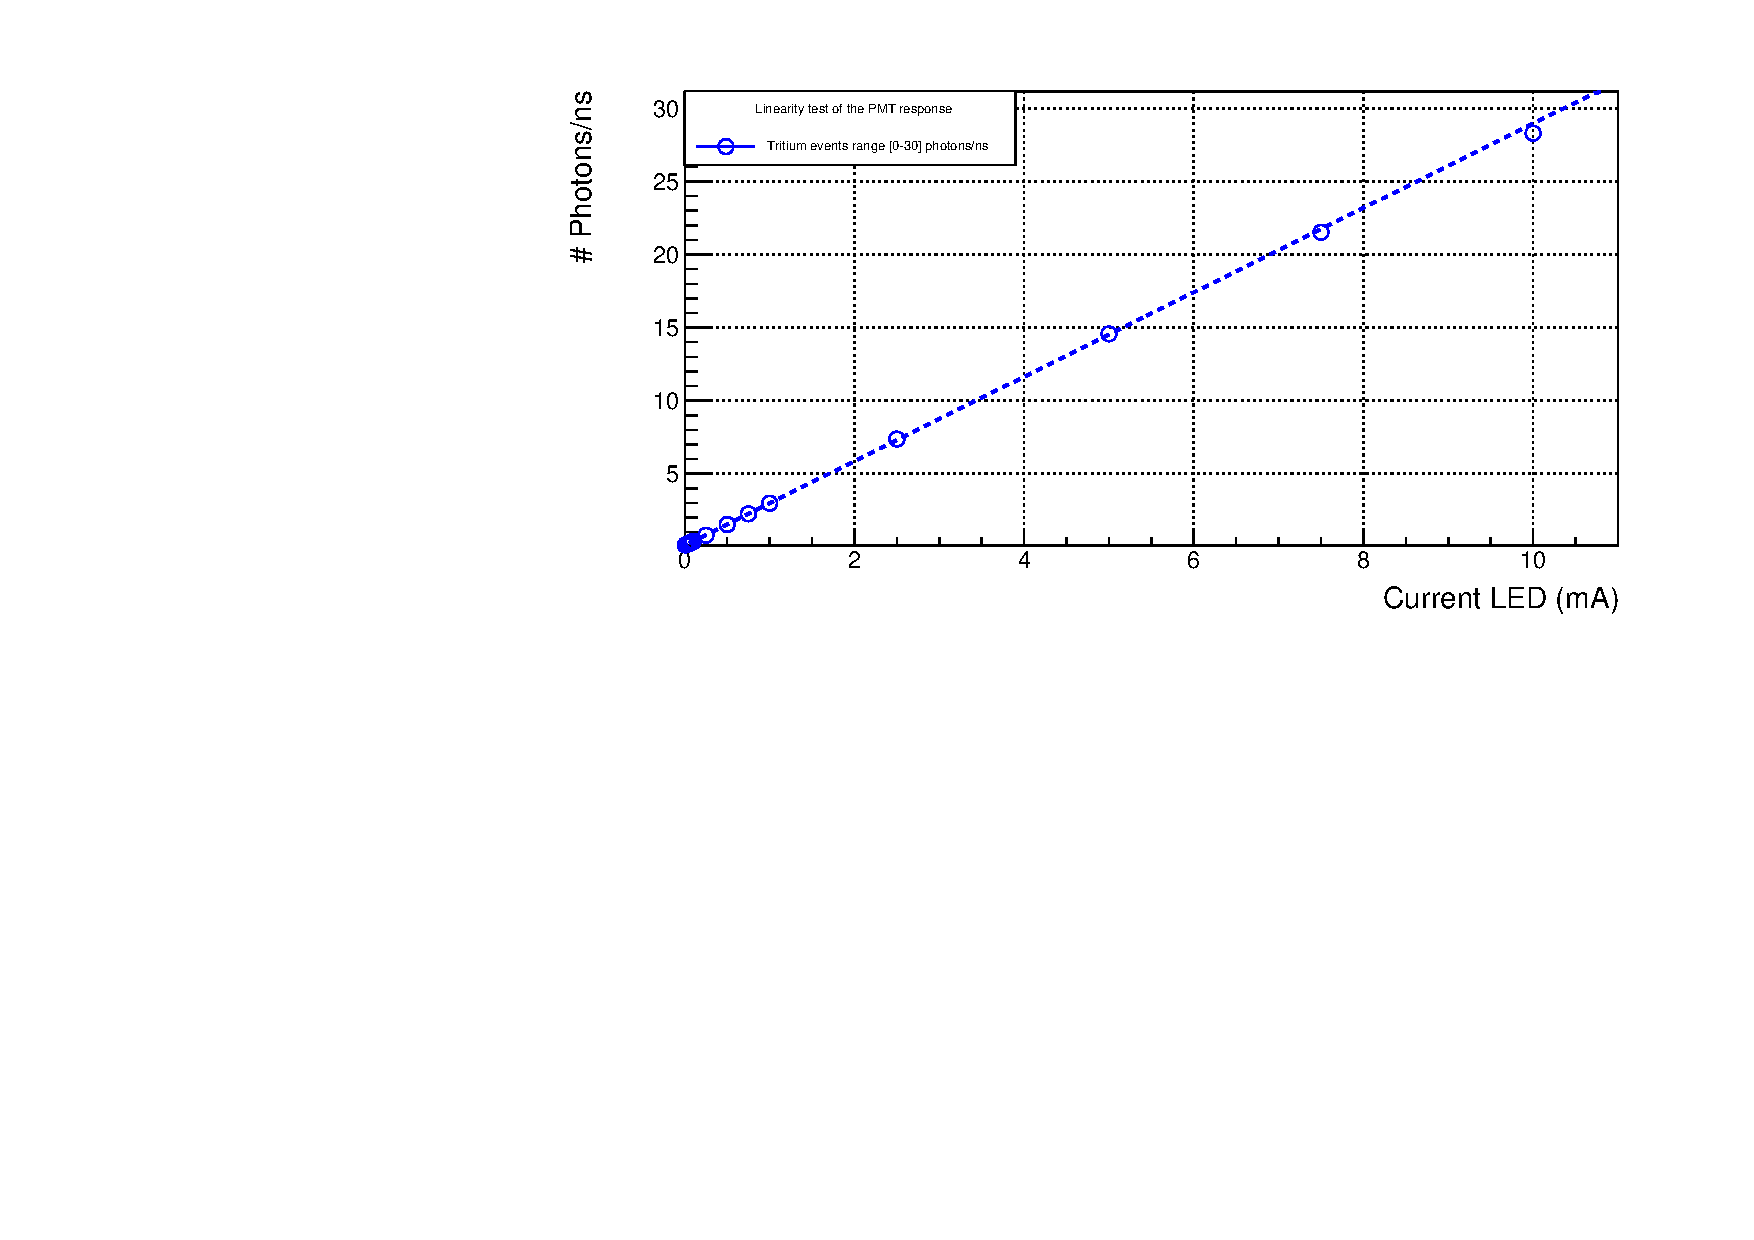
\includegraphics[width=0.8\textwidth]{4ResearchAndDevelopments/41Fibers/Linearity_test_0_30_range.pdf}}
    \newline
  \subfloat[Verification of linearity in the response of the PMT in the range of this study  $(0-2500)~\gamma/\nano\second$.]{
   \label{subfig:LinearityStudyRange}
    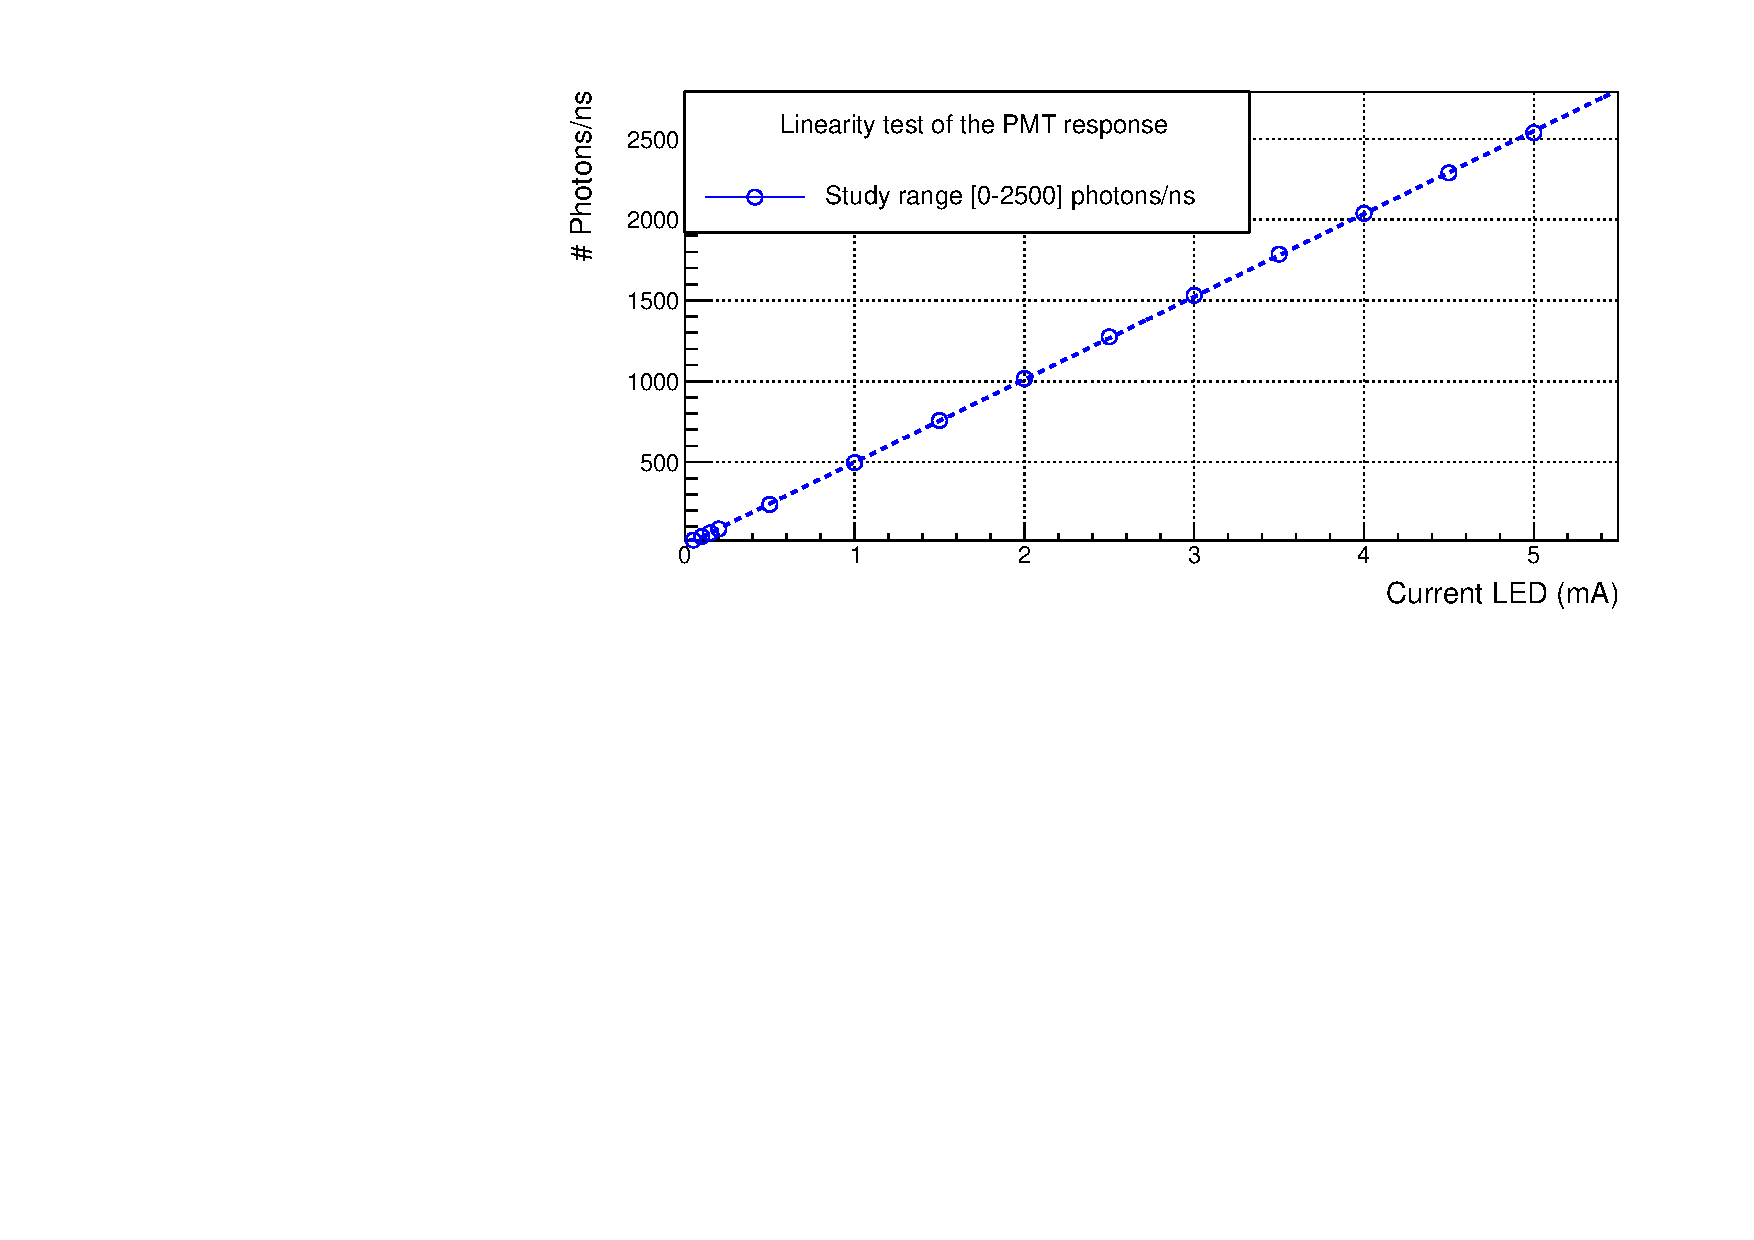
\includegraphics[width=0.8\textwidth]{4ResearchAndDevelopments/41Fibers/Linearity_test_0_2500_range.pdf}}
 \caption{Linearity tests of the PMT response}
 \label{fig:LinearityRangesOfPMT}
\end{figure}

As can be seen, the PMT output current is linear in both cases, so the system is ready to start with the characterization of the fibers.

First, the uncertainty of the conditioning process, $\sigma_{con}$, was experimentally measured. This uncertanty appeares because, as we have seen before, we have to condition each fiber, cutting and polishing it, before using and this is an individual task that can present a small dispersion, affecting the response of each individual fiber. It is an important measurement because this uncertainty will be present in the TRITIUM detector.

To measure it, we have to take into account that there is a bit of freedom in this system due to the position of the connectors which are fixed to the fiber ($1~\mm$ or less) which means that there is an additional uncertainty, $\sigma_{pos}$, in the measurement. Since both uncertainties are not related, the total measurement uncertainty can be calculated as a square sum, equation \ref{eq:TotalUncertaintyFiberCharacterization}.

\begin{equation}
\sigma_{t} = \sqrt{\sigma^2_{pos} + \sigma^2_{con} }
\label{eq:TotalUncertaintyFiberCharacterization}
\end{equation}

The uncertanty due to the fiber position are always presented in the measurement so, the only way we can measure the uncertainty due to the conditioning process is to quantify the uncertainty in the fiber position and extract it to the total uncertainty, sum of both, using the equation \ref{eq:ConditioningUncertaintyFiberCharacterization}. To do so we have designed two different experiments, one where only the uncertainty in the fiber position are presented ($\sigma_{t} = \sigma_{pos}$), and other in which only both uncertainties are involved.

\begin{equation}
\sigma_{con} = \sqrt{\sigma^2_{tot} - \sigma^2_{pos} }
\label{eq:ConditioningUncertaintyFiberCharacterization}
\end{equation}

The test designed to measure $\sigma_{pos}$ consisted of prepare one fiber of each type (no clad, single clad and multiclad) using the conditioning process explained before. Then, fix each fiber in the set up, take a measurement by feeding the LED at an intensity of $0.1~\milli\ampere$ and remove this fiber to the set up (and also the connectors). Finally, we repeat these measurements ten times with the same fiber, fixing and removing it every time.

With this test, we will obtain ten different measurements for each fiber type in which, the standard deviation of these measurements is only due to the uncertainty in the position. The results is shown in the table \ref{tab:PositionStandardDeviation}, whose results has been calculated using the equations \ref{eq:MeanAndStandardDesviation} and \ref{eq:RelativeStandardDesviation}.

\begin{equation}
Rel.~Std.~Des. = \frac{Std.Des.}{\bar{x}}
\label{eq:RelativeStandardDesviation}
\end{equation}

\begin{table}[htbp]
%%\centering
\begin{center}
\begin{tabular}{|c|c|c|c|c|}
\hline
Fiber type & Average ($\gamma$/ns) & Std. Des. ($\gamma$/ns) & Rel. Std. Des. (\%)\\
\hline \hline \hline
No Clad & $524.088 \pm 0.010$ & $17.65$ & $3.37$ \\ \hline
Single Clad & $1071.696 \pm 0.01$ & $9.07$ & $0.85$ \\ \hline
Multiclad & $949.930 \pm 0.026$ & $9.91$ & $1.04$ \\ \hline
\end{tabular}
\caption{Average and standard deviation (due to fiber position in setup) of photons per nanosecond that reach the PMT for $0.1~\milli\ampere$ LED intensity.}
\label{tab:PositionStandardDeviation}
\end{center}
\end{table}

As we can see, the clad of the fiber reduces the uncertainty due to the position of the fiber, which means that it improves the uniformity of the fiber response. Also, as can be seen from this table, the use of the clad greatly improves the collection efficiency of the fibers since both types of fibers with clad have collected more photons than the fiber without clad. A possible reason of that is because the photons are mainly collected in the core of the fiber and one of the most important things that will affect to the collection efficiency is the interface created by this core. 

This interface can be much more controlled in the case of a single clad or multiclad fibers where it is created between the core and the first clad, than in no clad fibers, where it is created between the core and the environment (air or water in our case), where external conditions, such as the dirt in the room, can affect a lot.

We can also see that the use of a second clad slightly reduce the collection efficienciy. A possible reason of that is ...

%We don't achieve any improvement with the second clad, which means that the photons are mainly collected in the core of the fiber.

%A possible reason of that is because, in the case of no clad fibers, the state of the interface between the core and the environment (air or water in our case) is much more important than in the others, where the most important interface is the one created between the fiber core and the first clad, which could be the reason why the difference between the signals of single clad and multiclad fibers are too small.

We can also see that the error of the measurement, provided by the keithley and propagated to the average, is three times smaller than the standard deviation, so we will not take it into account any more.

%In addition to the $\sigma_{pos}$ measurement, we have measured the number of photons collected by each type of fiber in the same situation, which is higher for single clad and even higher for multiclad. It means that the clad has an appreciable effect on the fiber collection efficiency and it could be a possible point to futur studies.

Now, we do the other experiment in which both uncertainties are involved. It consists of preparing ten different samples of each type of fiber (using the conditioning process) and measuring it under the same conditions as the previous test. This measurement will be done for four different LED emission intensities ($0.05$, $0.1$, $0.15$ and $0.2~\milli\ampere$) to reduce possibles mistakes.

The case of no clad fibers is shown in the figure \ref{fig:10samplesNC}, where we can see that, indeed, although each fiber shows a very linear trend with the amount of photons that it collects, a dispersion in the fiber response is clearly seen in each figure. Similar results were obtained for single clad and multiclad fibers.

%\begin{figure}[]
 %\centering
  %\subfloat[Number of photons/ns reaching the PMT for No Clad fibers.]{
   %\label{subfig:10samplesNC}
    %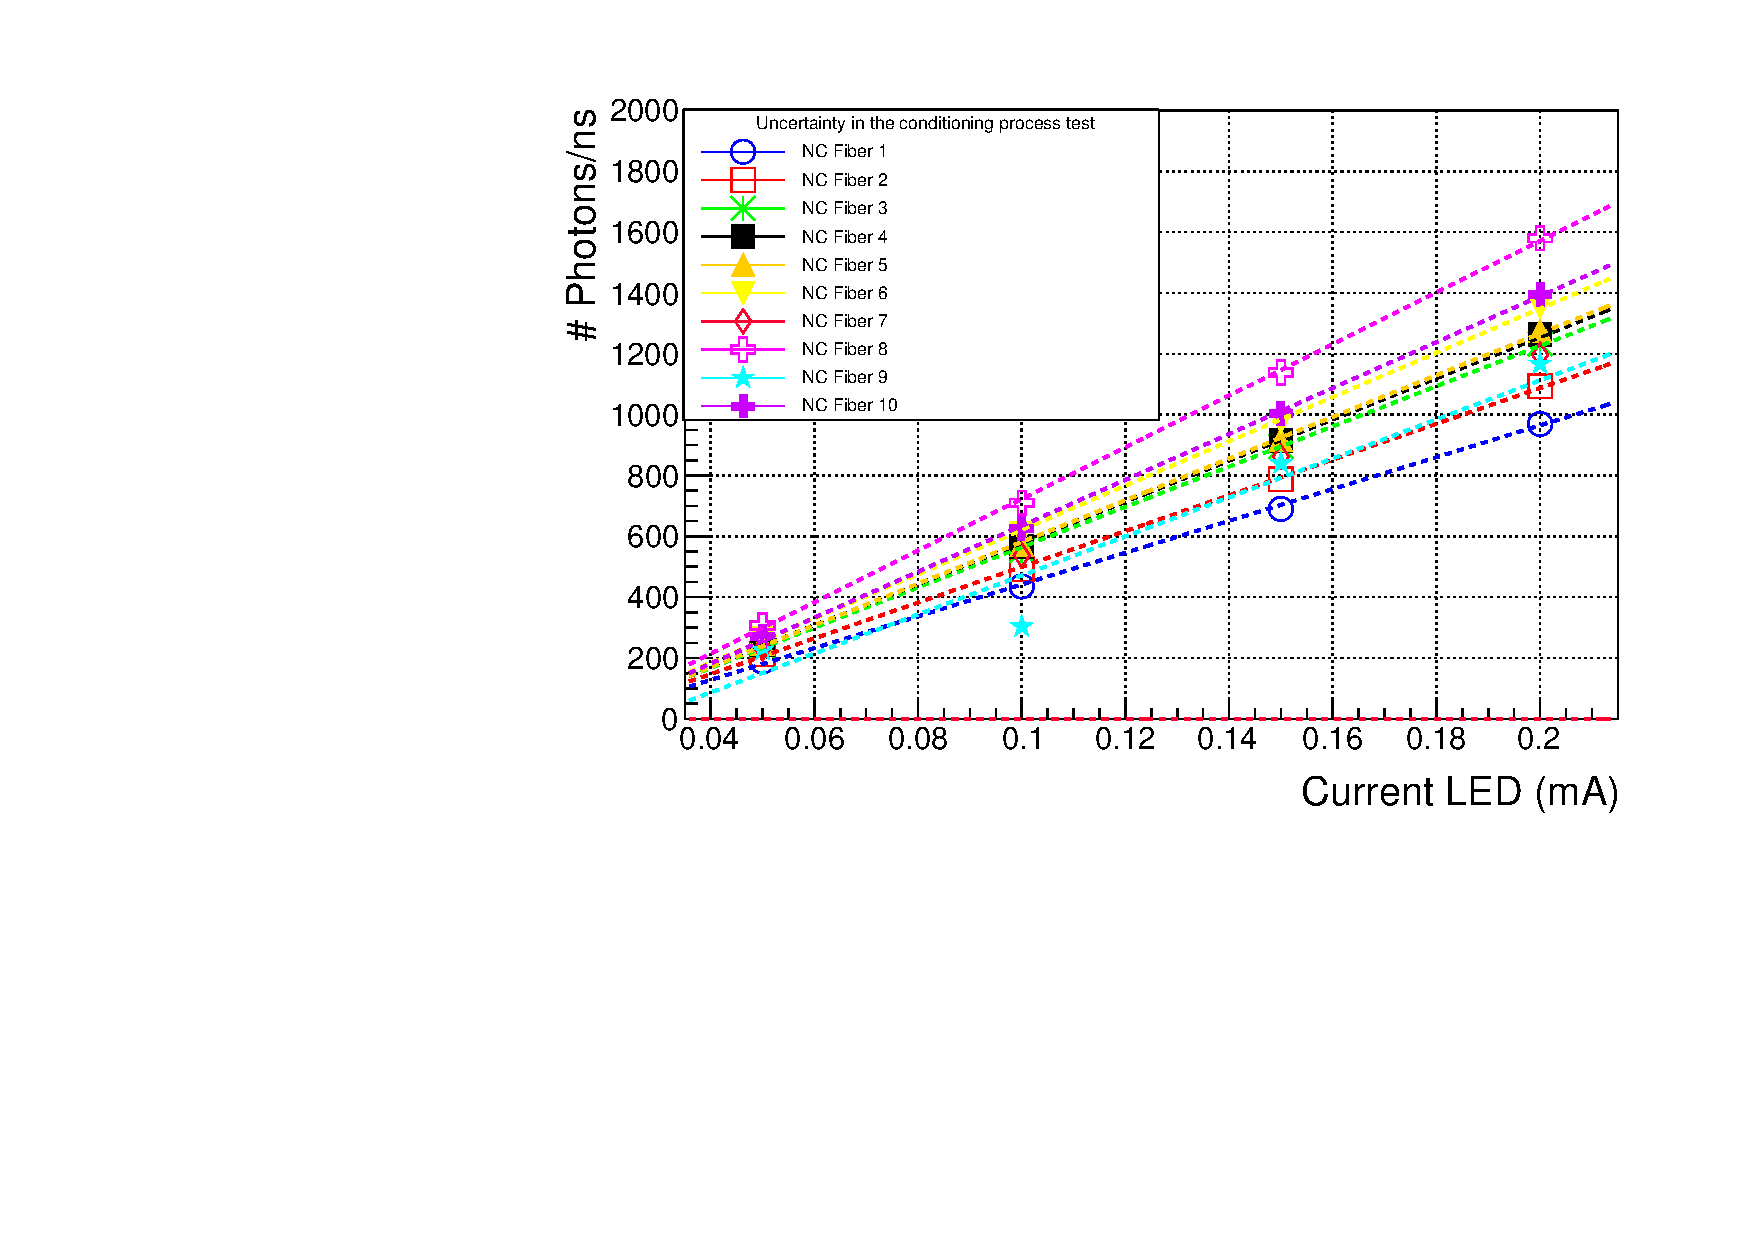
\includegraphics[width=0.75\textwidth]{4ResearchAndDevelopments/41Fibers/10_Different_samples_NoClad.pdf}}
    %\newline
  %\subfloat[Number of photons/ns reaching the PMT for Single Clad fibers.]{
   %\label{subfig:10samplesSC}
    %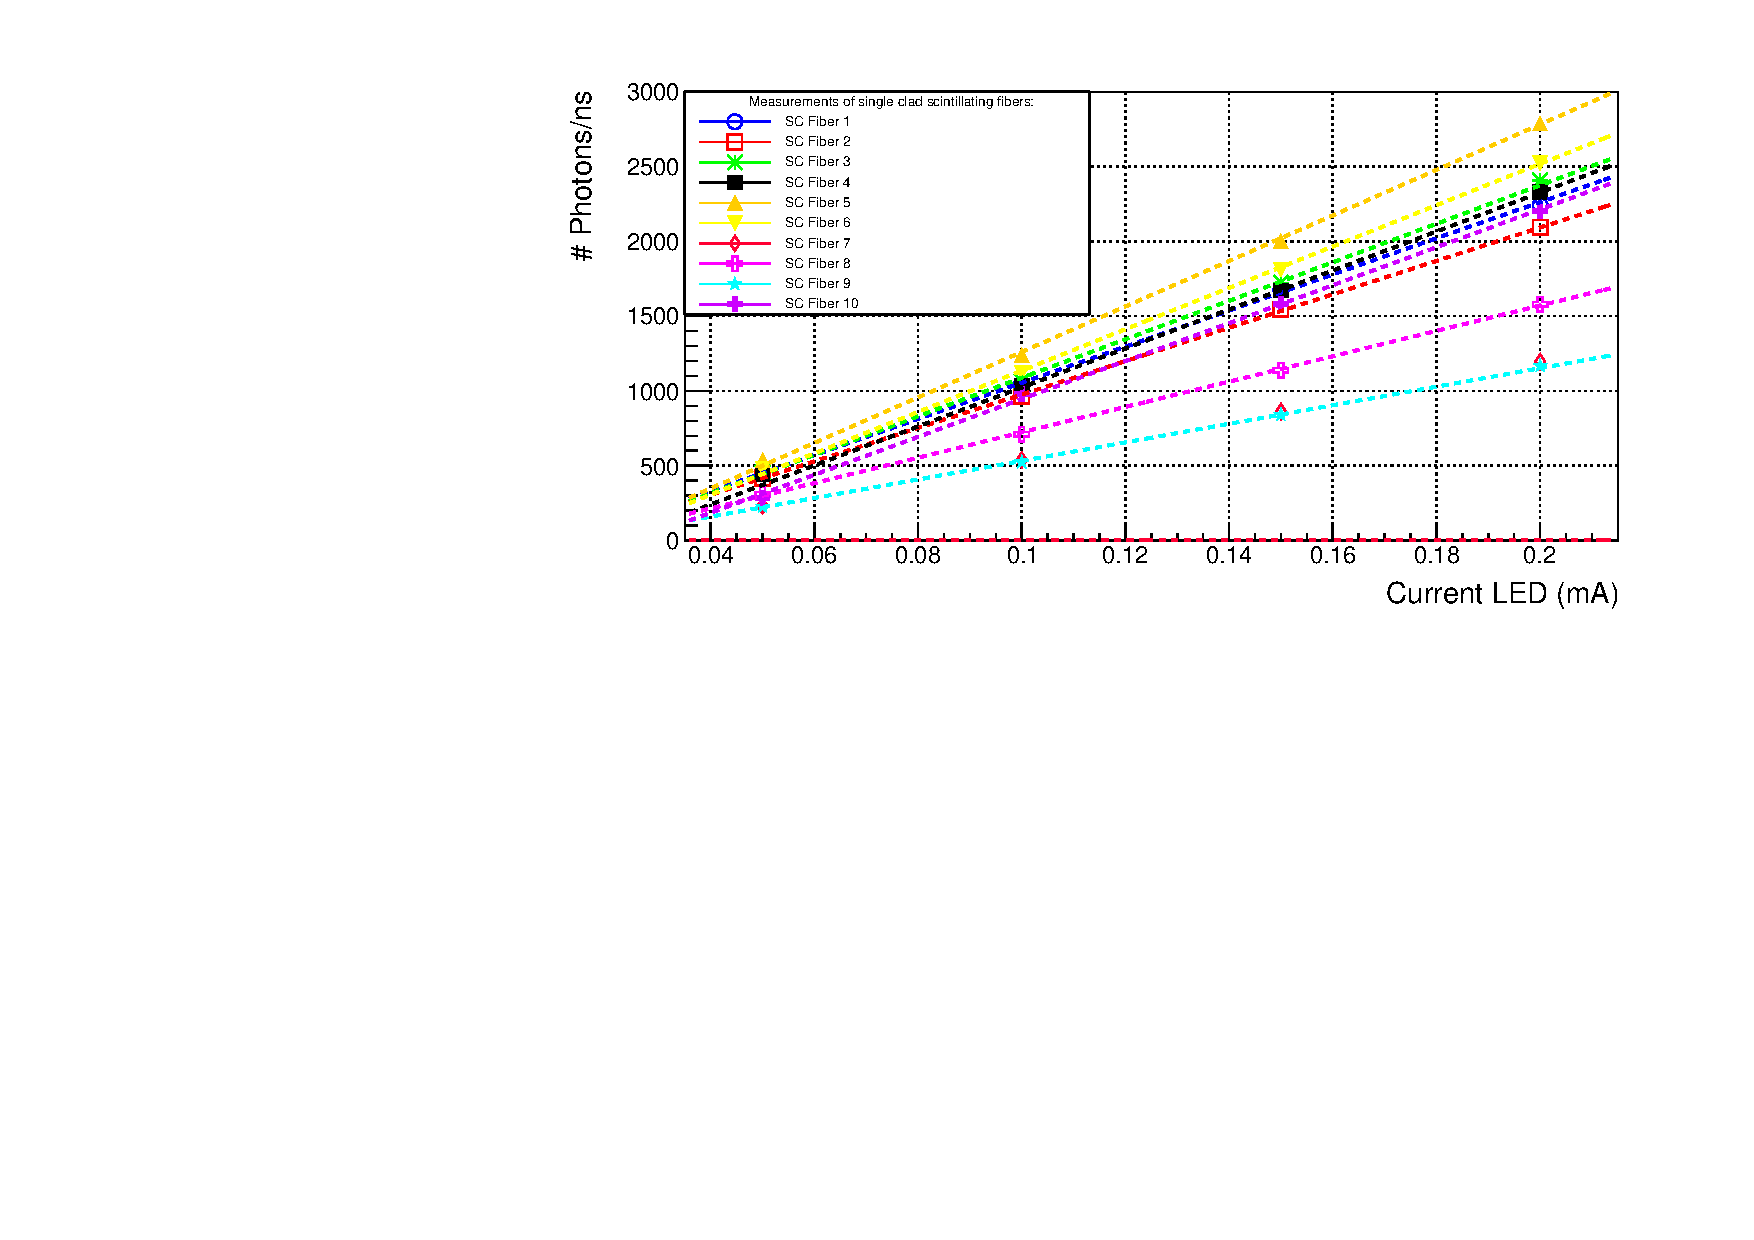
\includegraphics[width=0.75\textwidth]{4ResearchAndDevelopments/41Fibers/10_Different_samples_SingleClad.pdf}}
    %\newline
    %\subfloat[Number of photons/ns reaching the PMT for MultiClad fibers.]{
   %\label{subfig:10samplesMC}
    %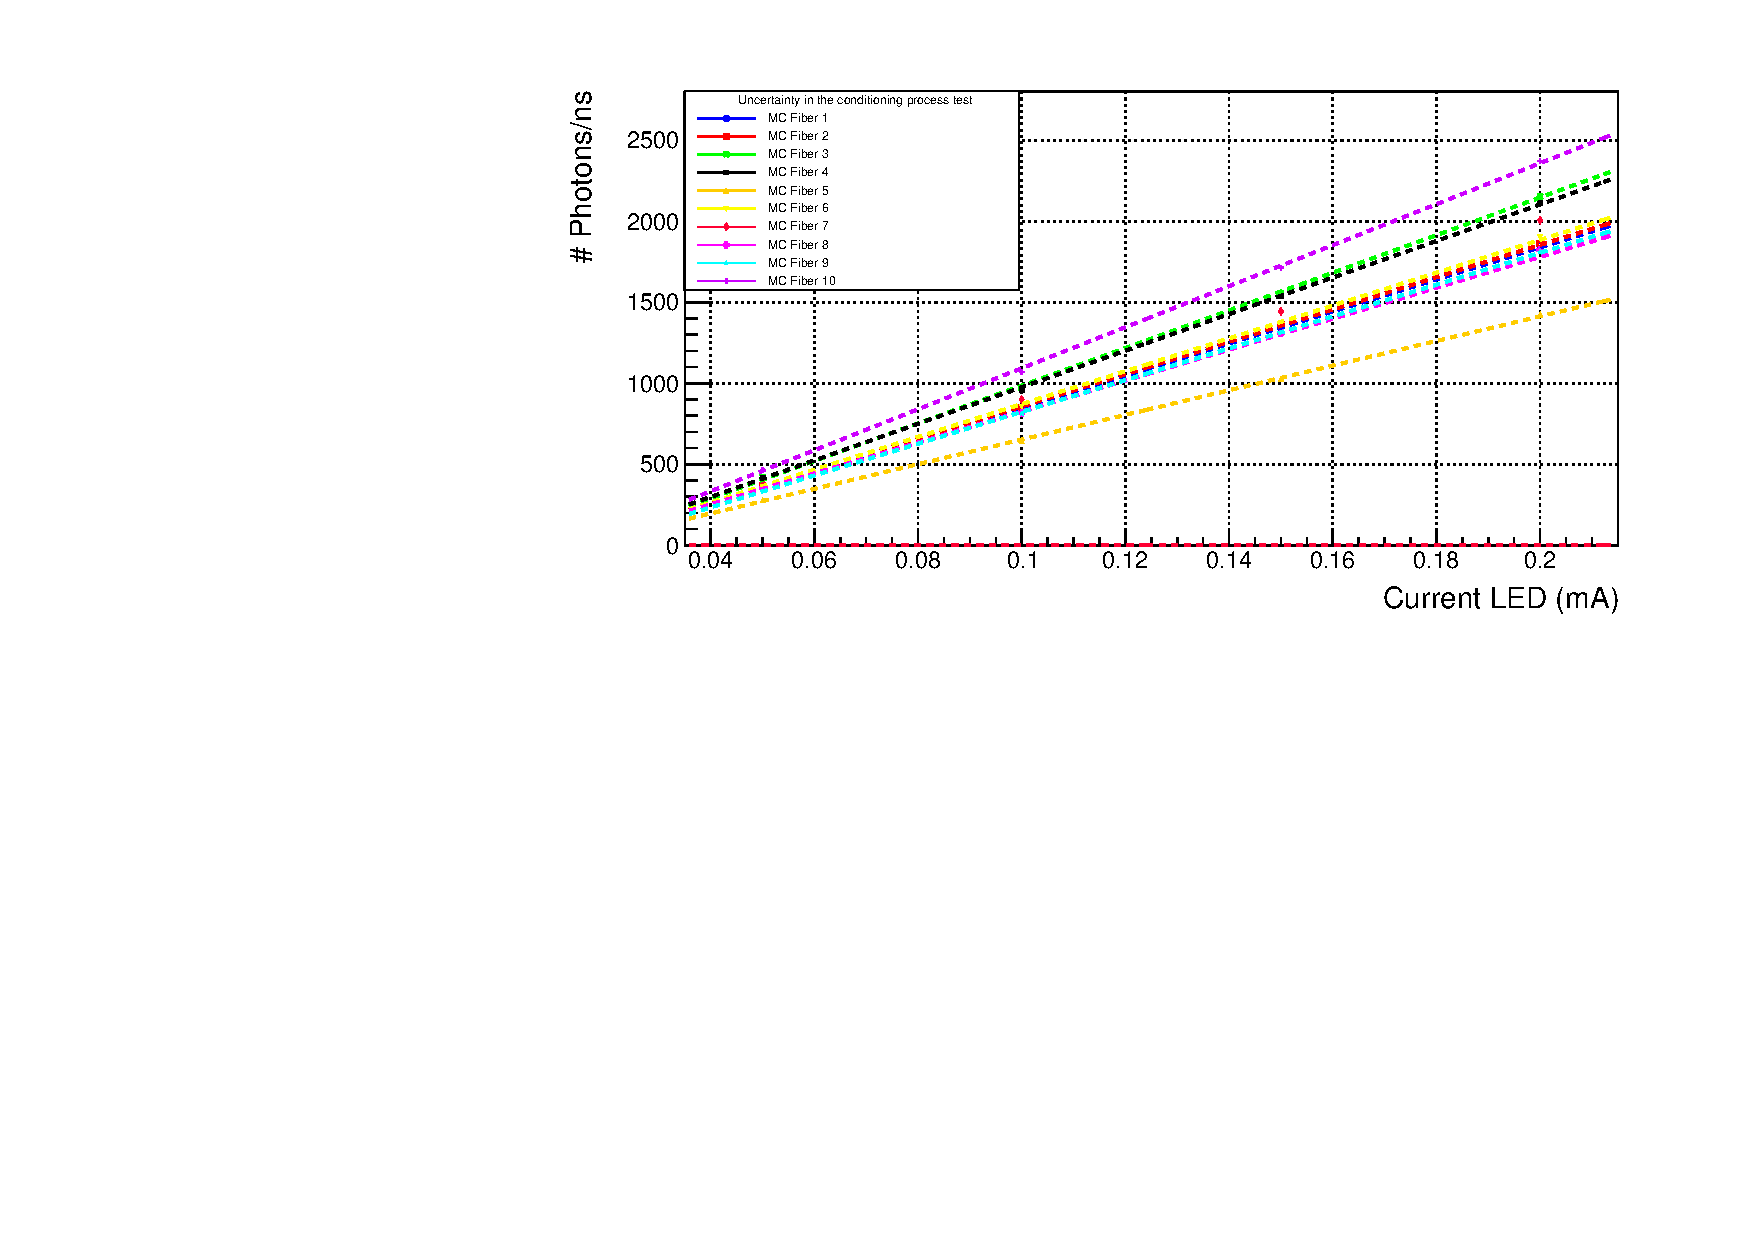
\includegraphics[width=0.75\textwidth]{4ResearchAndDevelopments/41Fibers/10_Different_samples_MultiClad.pdf}}    
 %\caption{Number of photons/ns reaching the PMT for ten samples of each fibers type.}
 %\label{fig:10samplesThreeTypes}
%\end{figure}


\begin{figure}[h]
\centering
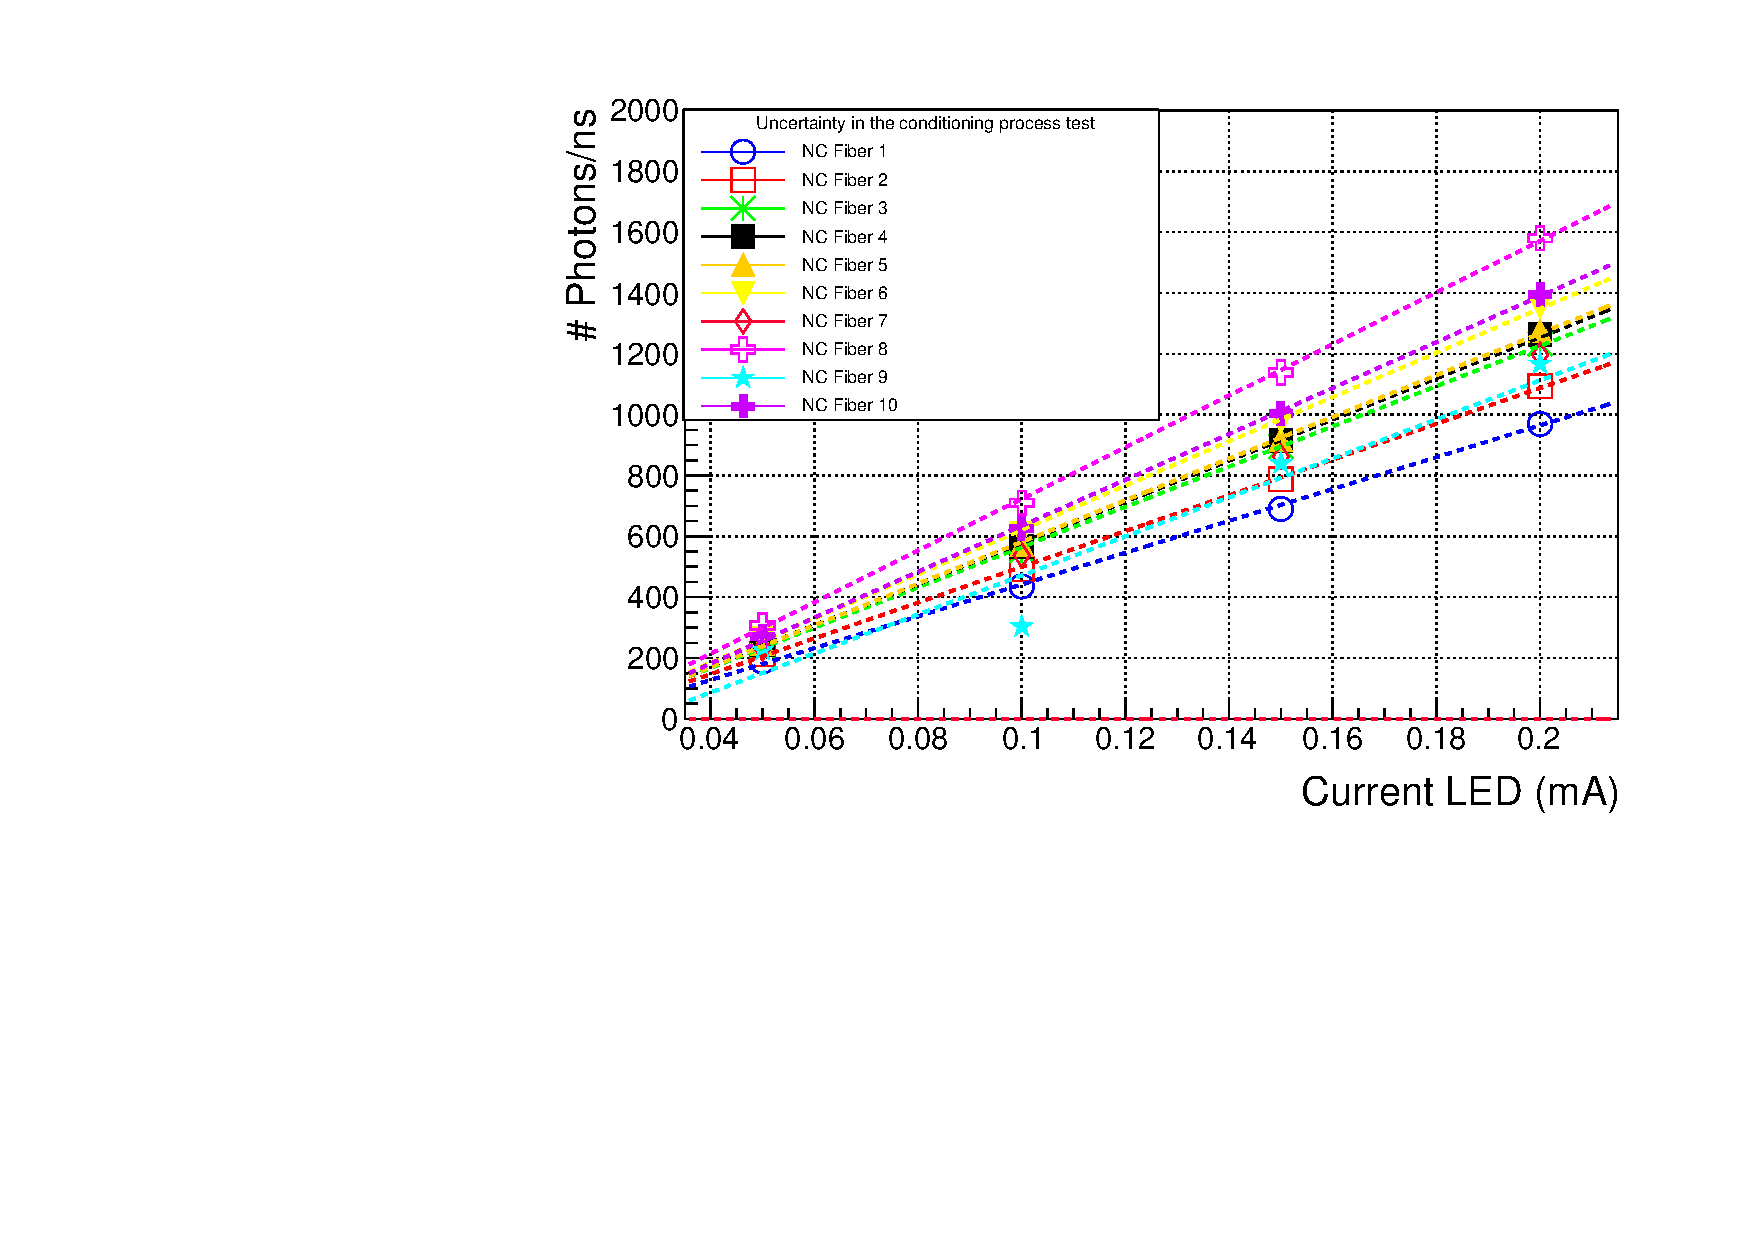
\includegraphics[scale=0.6]{4ResearchAndDevelopments/41Fibers/10_Different_samples_NoClad.pdf}
\caption{Number of photons/ns reaching the PMT for No Clad fibers.\label{fig:10samplesNC}}
\end{figure}

The average of these 10 samples for each type of fibers and its standard deviation are summarized in the tables \ref{tab:10DifferentSamplesNoClad}, \ref{tab:10DifferentSamplesSingleClad} and \ref{tab:10DifferentSamplesMultiClad} and represented in the figure \ref{fig:AveregeThreeFiberTypes}, where they can be compared. 

\begin{table}[htbp]
%%\centering
\begin{center}
\begin{tabular}{|c|c|c|c|c|}
\hline
Led Int. (mA) & Average ($\gamma$/ns) & Std. Des. ($\gamma$/ns) & Rel. Std. Des. (\%)\\
\hline \hline \hline
$0.05$ & $243.46$ & $9.82$ & $4.03$ \\ \hline
$0.1$ & $540.62$ & $33.51$ & $6.20$ \\ \hline
$0.15$ & $902.74$ & $36.83$ & $4.08$ \\ \hline
$0.2$ & $1252.62$ & $50.48$ & $4.03$ \\ \hline
\end{tabular}
\caption{Average, standard deviation and relative standard deviation of 10 different samples of no clad fibers.}
\label{tab:10DifferentSamplesNoClad}
\end{center}
\end{table}

\begin{table}[htbp]
%%\centering
\begin{center}
\begin{tabular}{|c|c|c|c|c|}
\hline
Led Int. (mA) & Average ($\gamma$/ns) & Std. Des. ($\gamma$/ns) & Rel. Std. Des. (\%)\\
\hline \hline \hline
$0.05$ & $383.81$ & $33.23$ & $8.66$ \\ \hline
$0.1$ & $922.68$ & $73.97$ & $8.02$ \\ \hline
$0.15$ & $1485.10$ & $119.90$ & $8.07$ \\ \hline
$0.2$ & $2053.78$ & $166.39$ & $8.10$ \\ \hline
\end{tabular}
\caption{Average, standard deviation and relative standard deviation of 10 different samples of single clad fibers.}
\label{tab:10DifferentSamplesSingleClad}
\end{center}
\end{table}

\begin{table}[htbp]
%%\centering
\begin{center}
\begin{tabular}{|c|c|c|c|c|}
\hline
Led Int. (mA) & Average ($\gamma$/ns) & Std. Des. ($\gamma$/ns) & Rel. Std. Des. (\%)\\
\hline \hline \hline
$0.05$ & $376.68$ & $14.96$ & $3.97$ \\ \hline
$0.1$ & $870.87$ & $34.58$ & $3.97$ \\ \hline
$0.15$ & $1396.60$ & $55.24$ & $3.95$ \\ \hline
$0.2$ & $1932.57$ & $76.02$ & $3.93$ \\ \hline
\end{tabular}
\caption{Average, standard deviation and relative standard deviation of 10 different samples of multi clad fibers.}
\label{tab:10DifferentSamplesMultiClad}
\end{center}
\end{table}

\begin{figure}[h]
\centering
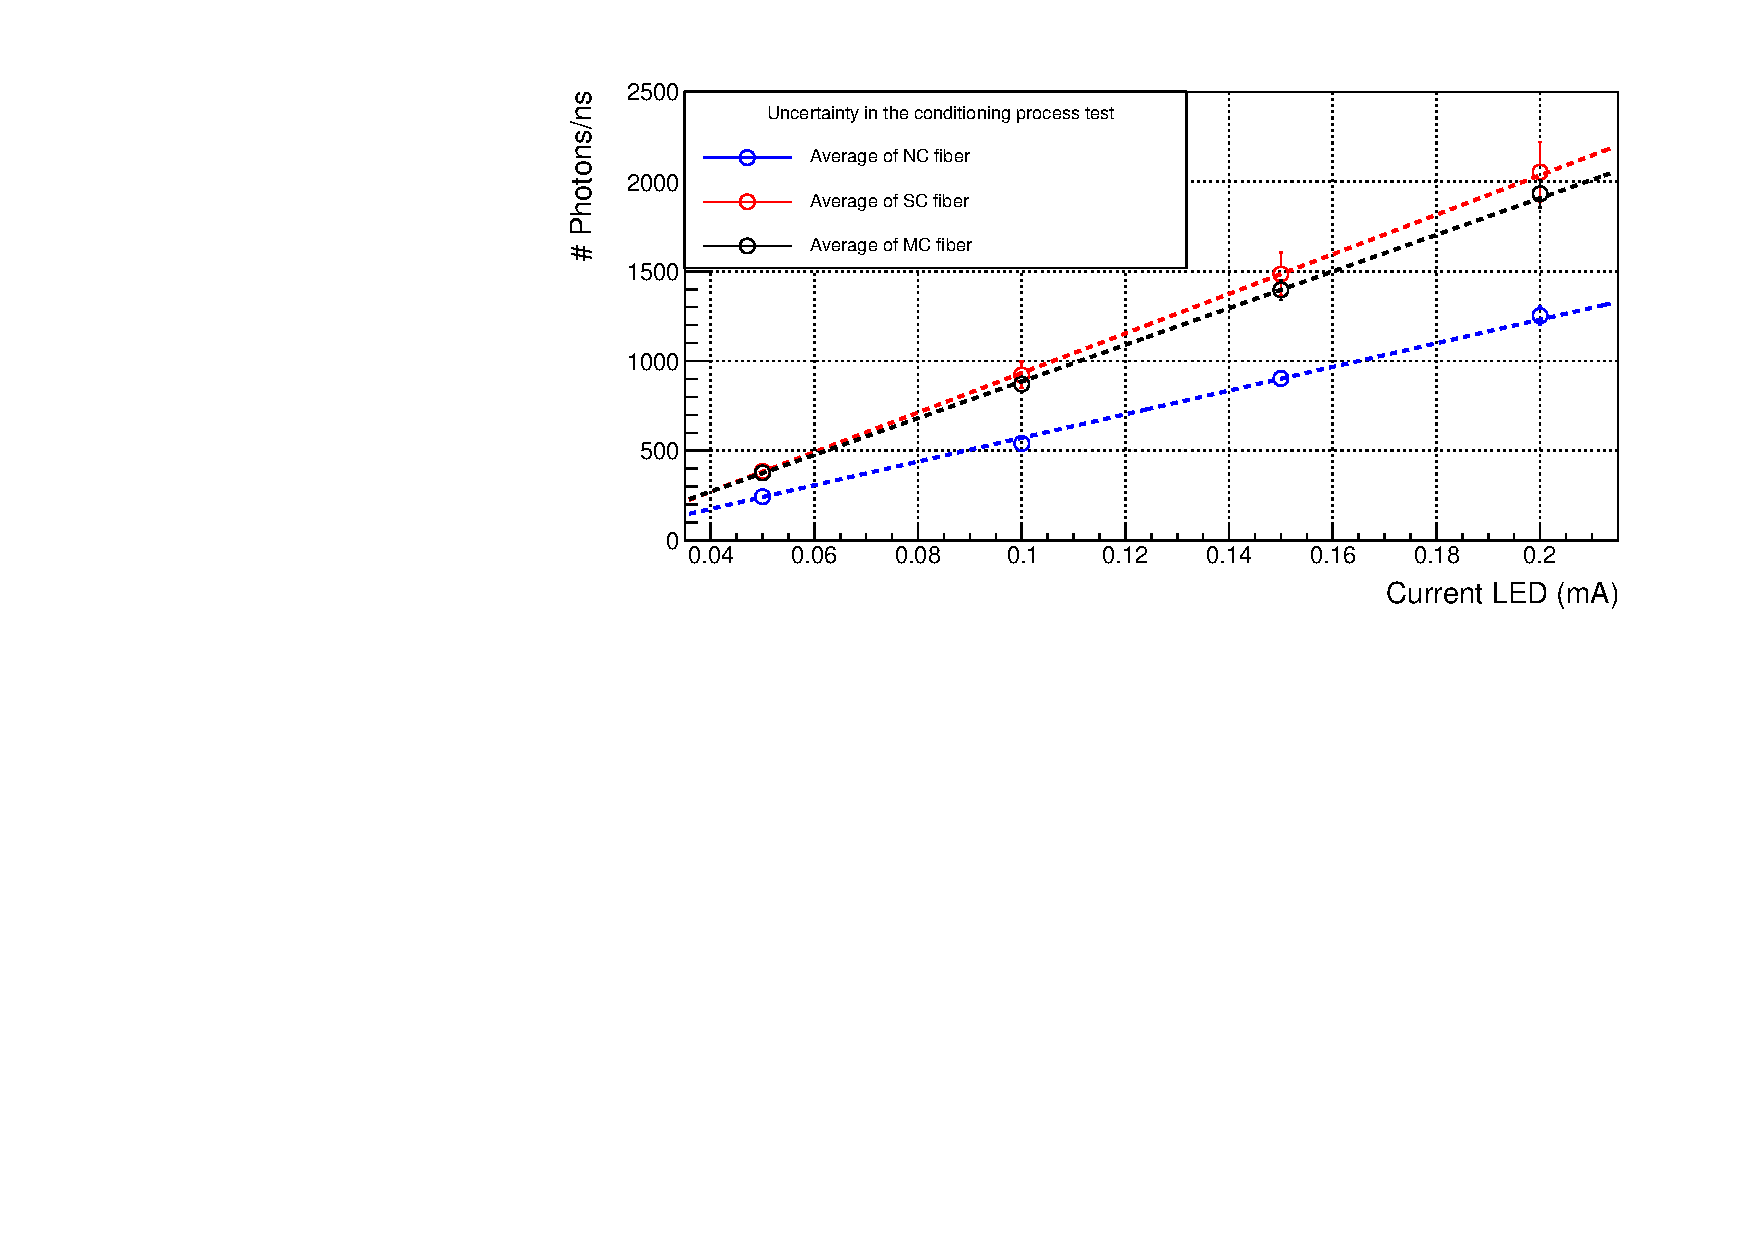
\includegraphics[scale=0.6]{4ResearchAndDevelopments/41Fibers/10_Different_Samples_Average_3_Fiber_Types.pdf}
\caption{Average of 10 samples for each fiber type (no clad, single clad and multiclad fibers).\label{fig:AveregeThreeFiberTypes}}
\end{figure}

As it is shown in the figure, they have a very linear trent which confirms the correct behavior of the fibers. We can also see that, similar to what happened with the previous test, single clad and multiclad fibers, both, have higher signals that no clad fibers, which means that the clad has an appreciable effect on the fiber collection efficiency and it could be a possible point to futur studies since, as we have said before, it is possible to develop our own fiber clad using the electrodeposition technique, with which we can create layers as thin as tens of nanometers.

Again, similar to what happened in the previous study, single-clad fibers have higher collection efficiency than multiclad fibers, something that has been verified in all our tests.

The relative standard deviation are also presented in these tables, where we can see that the dispersion of each fiber type for different LED intensities is practically negligible in each type of fiber, which again verifies the correct behavior of the system. 

There is only one point (no clad fiber with $0.1~\milli\ampere $) that is higher than we expect. We can see in the table \ref{tab:10DifferentSamplesNoClad} that the reason for this is that its standard deviation is too high (as high as the measurement for no clad fibers with $0.15~\milli\ampere$). The reason was found in the sample 9, whose measurement was very different from the average, incresing the standard deviation, probably because we did not wait enough time for system stabilization. We discard this sample because this result is not representative.

To uniform the results, an average of these four values is calculated for each fiber type and shown in table \ref{tab:RelativeStandardDeviations}, where the uncertainty in the fiber position, previously calculated, and the uncertainty due to the conditioning process, calculated using the equation \ref{eq:ConditioningUncertaintyFiberCharacterization}, are also shown. 

\begin{table}[htbp]
%%\centering
\begin{center}
\begin{tabular}{|c|c|c|c|}
\hline
Fiber type & $\sigma_t$ (\%) & $\sigma_{pos}$ (\%) & $\sigma_{con}$ (\%)\\\hline \hline \hline
No Clad & $4.01$ & $3.37$ & $2.17$ \\ \hline
Single Clad & $8.21$ & $2.17$ & $7.92$ \\ \hline
Multiclad & $3.96$ & $1.04$ & $3.82$ \\ \hline
\end{tabular}
\caption{Relative standard deviations ($\sigma_t$, $\sigma_{pos}$ and $\sigma_{con}$) measured in this test.}
\label{tab:RelativeStandardDeviations}
\end{center}
\end{table}

As we can see, the least uncertainty in the conditioning process is found in the no clad fibers, which means that the main damage from this process occurs in the fiber clad. It's something that was seen in figure \ref{fig:ResultofPolishingProcess}. It has been seen under the microscope that this damage only occurs at the end of the fiber, where we cut and polish it.

Also, the largest relative standard deviation in this process is recorded for single clad fibers, which means that the second clad increases the resistance of the fiber to this process.

In summary, as a result of these tests we have seen that, on the one hand, the use of fiber clad improves the photon collection efficiency, which could be an interesting point for future studies. As we have said before, it is possible to develop our own fiber clad using the electrodeposition technique, with which we can create layers as thin as tens of nanometers.

On the other hand, we have quantified the relative statistical deviation due to the fiber conditioning process developed in the TRITIUM experiment, where it has been seen that the fiber clad is the main damage of this conditioning process so, if we want to develop a method to create our own clad, it should be applied after the fiber conditioning process.

Finally, the measurement of the photon collection efficiency of each type of fiber is shown. The collection efficiency is the percentage of photons collected along the fibers. It is usually given by the manufacturer per meter of fiber, $ EC_ {100} $.

To measure it, we prepare ten different samples of $10~\cm$ in length for each type of fiber and measure each one using the set up previously explained. Then, the average and standard deviation was calculated for each type of fiber using the equations \ref{eq:MeanAndStandardDesviation}, whose results are shown in table \ref{tab:10DifferentSamplesAlltypes}.

\begin{table}[htbp]
%%\centering
\begin{center}
\begin{tabular}{|c|c|c|c|c|}
\hline
Led Int. (mA) & No clad ($\gamma$/ns) & Single clad ($\gamma$/ns) & MultiClad ($\gamma$/ns) \\
\hline \hline \hline
$0.05$ & $318.35 \pm 61.34$ & $549.62 \pm 70.79$ & $480.35 \pm 83.72$ \\ \hline
$0.1$ & $735.65 \pm 143.02$ & $1269.91 \pm 164.32$ & $1110.66 \pm 193.44$ \\ \hline
$0.15$ & $1183.91 \pm 232.07$ & $1983.93 \pm 230.97$ & $1777.40\pm 307.19$ \\ \hline
$0.2$ & $1645.18 \pm 323.76$ & $2506.97 \pm 208.01$ & $2338.43 \pm 350.24$ \\ \hline
\end{tabular}
\caption{Average and standard deviation of 10 different fibers of $10~\cm$.}
\label{tab:10DifferentSamplesAlltypes}
\end{center}
\end{table}

The collection efficiency can be calculated by comparing these tests with those performed for a fiber length of $20~\cm$, whose values has been previously shown in the tables \ref{tab:10DifferentSamplesNoClad}, \ref{tab:10DifferentSamplesSingleClad} and \ref{tab:10DifferentSamplesMultiClad} since both have been made under the same conditions. The results is shown in the table \ref{tab:CollectionEfficiencyOfFibers}:


%Due to the reason that both tests were run in the same setup under exactly the same conditions, the difference between both situations is the photons per nanosecond that have not been collected in this extra $10~\cm$ of fiber. Therefore, using the equation \ref{}, the collection efficiency in $10~\cm$ of fiber can be calculated for each sort of fiber, whose result is shown in the last column.

\begin{table}[htbp]
%%\centering
\begin{center}
\begin{tabular}{|c|c|c|}
\hline
Fiber type & $CE_{10}$ (\%) & $CE_{100}$ (\%) \\\hline \hline \hline
No Clad & $75.97 \pm 7.61$ & $7.597 \pm 0.761$ \\ \hline
Single Clad & $77.96 \pm 5.66$ & $7.796 \pm 0.566$ \\ \hline
Multiclad & $82.60 \pm 7.24$ & $8.260 \pm 0.724$ \\ \hline
\end{tabular}
\caption{Collection efficiency of each fiber type for 10 centimeters, $CE_{10}$, and 1 meter, $CE_{100}$.}
\label{tab:CollectionEfficiencyOfFibers}
\end{center}
\end{table}

We have to keep in mind that the difference between the fiber length in both studies is only $10~\cm$, so the collection efficiency calculated from these measurements, $CE_{10}$, is only at that distance. The collection efficiency is normally given at a distance of one meter so, assuming that this parameter has a linear dependence with the distance, we can extrapolate it, whose value is shown in the last column, $CE_{100}$.

The collection efficiency per meter given by the manufacturer Saint Gobain is between 7\% and 3.44\% \cite{DataSheetBCF12Fiber}. We are using collimated photons for that so we can guess that we are in the best situation, 7\%. 

As can be seen in the table \ref{tab:CollectionEfficiencyOfFibers}, our measured values are very close to the one provided by the manufacturer. The difference between this value for the three types of fiber studied is not as great as we expect. We have to take into account that we are using a difference in fiber length of only $10~\cm$ and it may not be enough to see this effect. It might be interesting to repeat these tests with a greater difference in fiber length.